% A skeleton file for producing Computer Engineering reports
% https://github.com/DeepHorizons/KGCOEReport_template

\documentclass[CMPE]{KGCOEReport}

% The following should be changed to represent your personal information
\newcommand{\classCode}{CMPE 460}  % 4 char code with number
\newcommand{\name}{Jacob Meyerson}
\newcommand{\LabSectionNum}{2}
\newcommand{\LabInstructor}{Professor Beato}	
\newcommand{\TAs}{Brunon Sztuba \\ Eri Montano \\ Connor Henley}
\newcommand{\LectureSectionNum}{1}
\newcommand{\LectureInstructor}{Professor Beato}
\newcommand{\exerciseNumber}{2}
\newcommand{\exerciseDescription}{UART Driver}
\newcommand{\dateDone}{February 05, 2021}
\newcommand{\dateSubmitted}{February 12, 2021}

\usepackage{float}
\usepackage{titlesec}
\usepackage{pdfpages}

\begin{document}
\maketitle

\iffalse % No table of contents or other sections for a worksheet -------------------------------------------------
\tableofcontents	%Make a table of contents for all of the sections
\newpage			%New page after table of contents

%Abstract Section
\section*{Abstract}
\addcontentsline{toc}{section}{Abstract}
		
%Design Methodology Section
\section*{Design Methodology}
\addcontentsline{toc}{section}{Design Methodology}

%Results Section	
\section*{Results \& Analysis}
\addcontentsline{toc}{section}{Results \& Analysis}

%Conclusion Section
\section*{Conclusion}
\addcontentsline{toc}{section}{Conclusion}

\fi % -------------------------------------------------------------------------------------------------------------------------------

\section*{Lab Description}
The purpose of this lab is to implement methods to transmit and receive data in the form of characters through UART (Universal asynchronous receiver-transmitter). By polling flags in the UART status registers, characters are either sent or received through a serial console with the K64. 

% Screenshots
\section*{Screenshots}

\begin{figure}[H]
	\centering
  	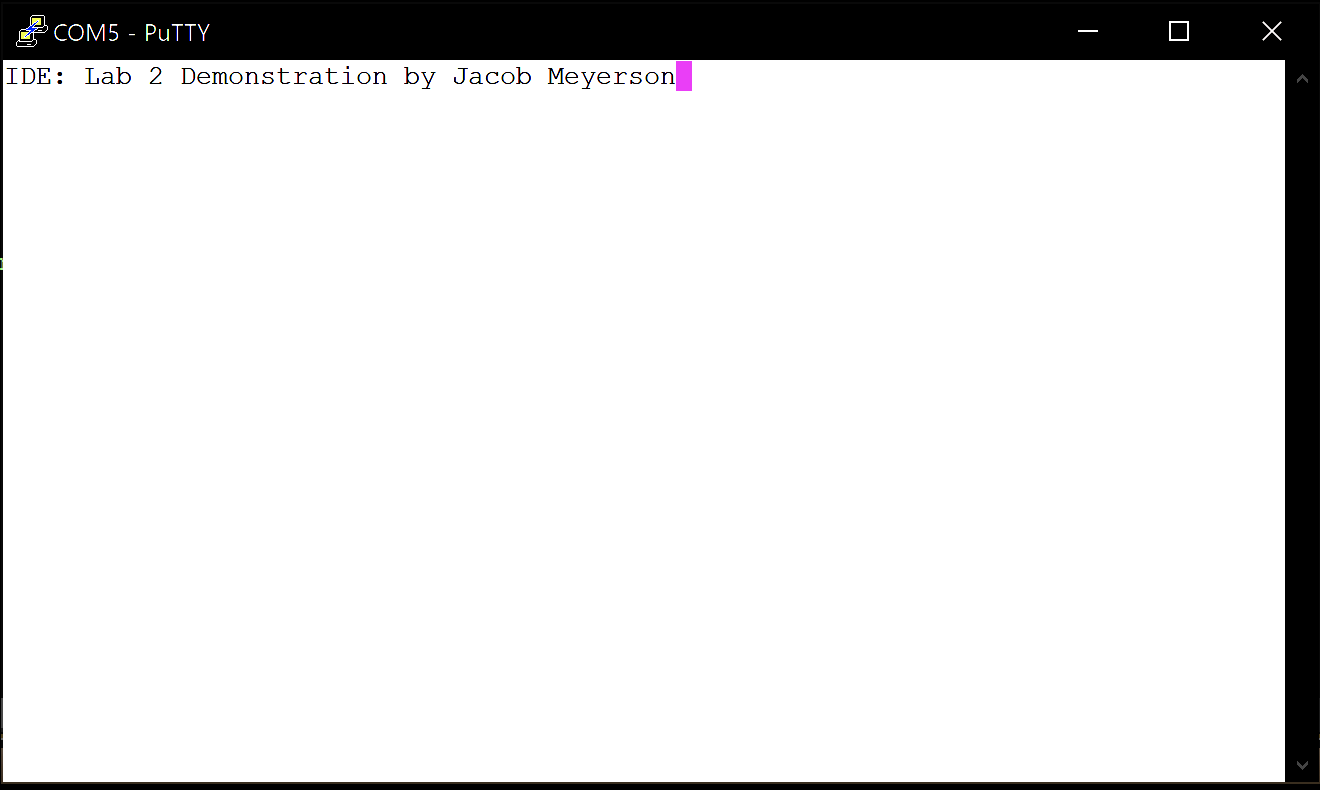
\includegraphics[width=1.0\textwidth]{Screenshots/UART_lab_part_2}  
	\caption{UART Driver Demo Part 2}
	\label{Figure 1}
\end{figure}

\begin{figure}[H]
	\centering
  	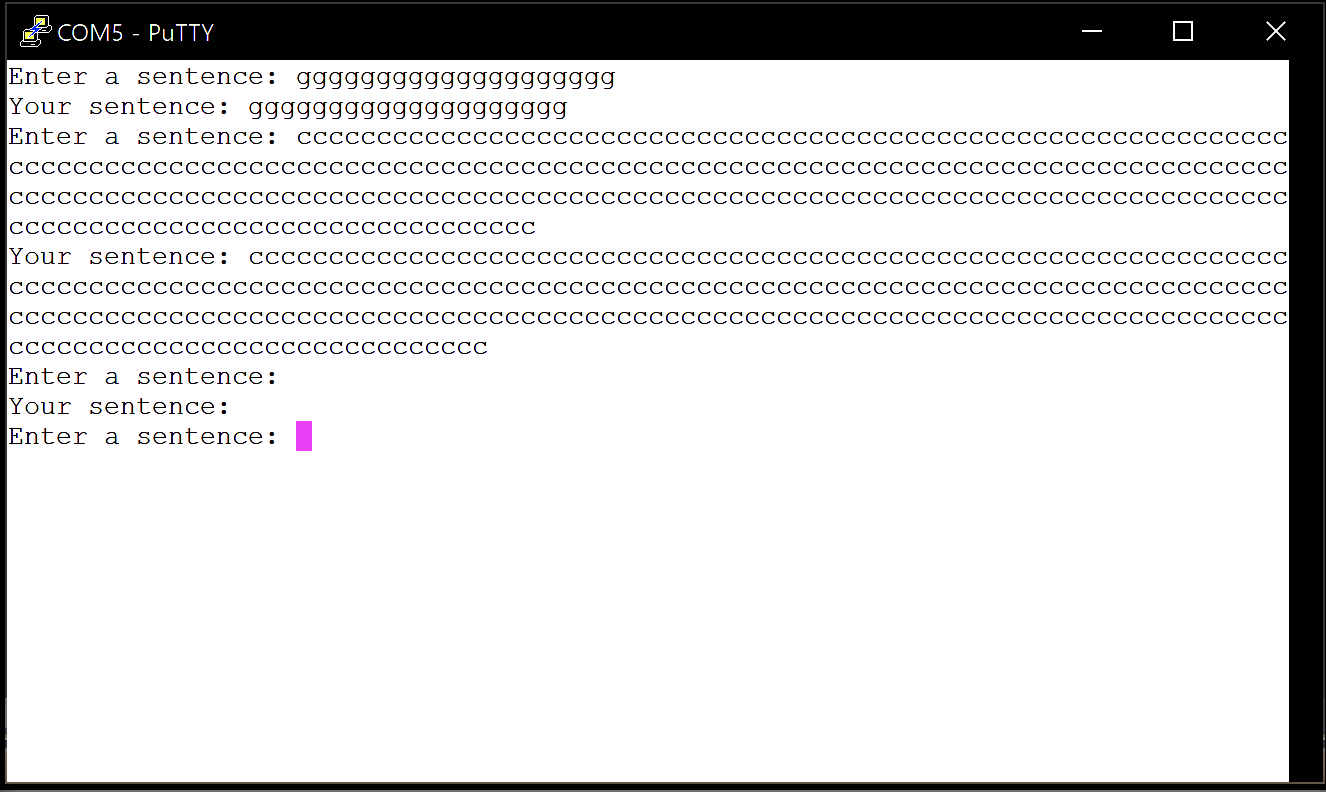
\includegraphics[width=1.0\textwidth]{Screenshots/UART_lab_part_3}  
	\caption{UART Driver Demo Part 3}
	\label{Figure 2}
\end{figure}

\newpage
\includepdf[pages=-,pagecommand={},width=\paperwidth]{Screenshots/lab2_signoff.pdf}

\end{document}